\scanpage{106}
ayant les propriétés suivantes
\[
\text{a)}\quad N(x_1\otimes x_2)=N_{A_1}(x_1)N_{A_2}(x_2)
\qquad\begin{gathered}x_1\in\Gamma A_1\\x_2\in\Gamma A_2\end{gathered}
\]
\[
\text{b)}\quad \varphi_N(\xi,\eta)=\operatorname{Tr}_{A_1\otimes A_2/A}(\xi\bar\eta)
\]
\deleted{On aura de}
i.e.
\[
 \deleted{\unsure{\varphi}}N(\xi+\eta)=N(\xi)+N(\eta)+\operatorname{Tr}(\xi\bar\eta)
\]
On \deleted{aura alors}, pour $\forall\xi\in A_1\otimes A_2$
\[
 \boxed{i(N(\xi))=\xi\bar\xi}
\]
\[
\left\{\boxed{\begin{gathered}
 N(\sigma_1\otimes\operatorname{id}_{A_2}(\xi))=N(\operatorname{id}_{\unsure{A_2|A_1}}\otimes\sigma_2(\xi))=\overline{N(\xi)}\\
 N(\bar\xi)=N(\xi)
\end{gathered}}\right.
\]
\margin{\unsure{Noter} aussi $\boxed{N_{A_1\otimes A_2/A}(i(\eta))=\eta^2}$.}
De plus, on a
\[
 \boxed{N_{A/O}\bigl(N_{A_1\otimes A_2/A}(\xi)\bigr)=N_{A_1\otimes A_2/O}(\xi)}
\]
sans compter la formule plus bénigne
\[
 \boxed{\operatorname{Tr}_{A/O}\bigl(\operatorname{Tr}_{A_1\otimes A_2/A}(\xi)\bigr)=\operatorname{Tr}_{A_1\otimes A_2/O}(\xi)}
\]
Prouvons p.ex. la première des deux dernières. La \deleted{deuxième}
Posons
\[
 \sigma_1=\sigma_{A_1}\otimes\operatorname{id}_{A_2},\qquad
 \sigma_2=\operatorname{id}_{A_1}\otimes\sigma_2,
 \qquad\sigma_3=\sigma_1\sigma_2
\]
\deleted{\unsure{\xi}}\deleted{Soit} $\xi=\xi_0\in A$, \deleted{on doit vérifier}
\inserted{$\xi_i=\sigma_i(\xi)$,}
on \unsure{constate} qu'on \unsure{ait|a}
\figure{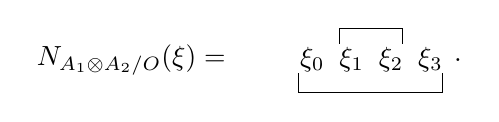
\begin{tikzpicture}
\node at (0,0) {$N_{A_1\otimes A_2/O}(\xi)=$};
\node at (2.3,0) {$\xi_0$};
\node at (2.8,0) {$\xi_1$};
\node at (3.3,0) {$\xi_2$};
\node at (3.8,0) {$\xi_3$};
\node at (4.15,0) {$.$};
\draw (2.12,-.17)--(2.12,-.42)--(3.95,-.42)--(3.95,-.17);
\draw (2.65,.2)--(2.65,.4)--(3.45,.4)--(3.45,.2);
\end{tikzpicture}}
\mspage{105}
